\section*{Part B -- Graph Essentials and Measures (70 pts): Q3 and Q4}

\subsection*{Q3: Graph Creation (10 pts)}

The edge list \texttt{graph.txt} (attached to this assignment as
\texttt{graph-1.txt}) contains $26{,}377$ tab-separated lines, each giving one
undirected edge. It was loaded into a simple undirected graph
(\texttt{networkx.Graph}), adding one node per distinct identifier appearing in
the file and one edge per line; no isolated nodes were added and the file was
not symmetrised a second time. The file contains no self-loops and no duplicate
edge in either orientation, so the $26{,}377$ lines yield exactly $26{,}377$
distinct edges.

\begin{table}[ht]
  \centering
  \begin{tabular}{lr}
    \toprule
    Quantity & Value \\
    \midrule
    Number of nodes                & $26{,}728$ \\
    Number of edges                & $26{,}377$ \\
    Number of connected components & $4{,}104$  \\
    \bottomrule
  \end{tabular}
  \caption{Q3: basic counts for the graph built from the edge list.}
  \label{p2:tab:q3}
\end{table}

\noindent\textbf{Answer.} The graph has \textbf{26{,}728 nodes},
\textbf{26{,}377 edges} and \textbf{4{,}104 connected components}.

The graph is therefore very sparse (mean degree $2m/n \approx 1.97$) and highly
fragmented. It is not a forest: a forest on $n$ nodes with $c$ components would
have $n-c = 26{,}728-4{,}104 = 22{,}624$ edges, whereas the graph has
$26{,}377$, so it carries $m-n+c = 3{,}753$ independent cycles.

\subsection*{Q4(a): Largest connected component (10 pts)}

Connected components were extracted with
\texttt{nx.connected\_components} and sorted by size in decreasing order; the
largest is the first element. Its edge count is that of the \emph{induced}
subgraph on those nodes, not the edge count of the whole graph.

\begin{table}[ht]
  \centering
  \begin{tabular}{lrr}
    \toprule
    Component & Nodes & Edges \\
    \midrule
    Largest (LCC)        & $13{,}903$ & $16{,}695$ \\
    Second largest       & $69$       & $80$       \\
    \midrule
    Whole graph          & $26{,}728$ & $26{,}377$ \\
    \bottomrule
  \end{tabular}
  \caption{Q4: size of the two largest connected components, against the whole
  graph.}
  \label{p2:tab:q4}
\end{table}

\noindent\textbf{Answer.} The largest connected component has
\textbf{13{,}903 nodes} and \textbf{16{,}695 edges}. It is a giant component in
the usual sense: it holds $52.0\%$ of all nodes and $63.3\%$ of all edges, while
the remaining $4{,}103$ components share the other half of the nodes.

\subsection*{Q4(b): Visualization of the second largest connected component (10 pts)}

\paragraph{Which component, and how it was selected.}
The components were sorted by node count in decreasing order and the element at
index $1$ was taken, i.e.
\begin{center}
\texttt{sorted(nx.connected\_components(G), key=len, reverse=True)[1]}.
\end{center}
The ten largest component sizes are
\[
  13{,}903,\; \mathbf{69},\; 30,\; 30,\; 29,\; 26,\; 23,\; 21,\; 21,\; 20 .
\]
\textbf{There is no tie for second place}: exactly one component has $69$ nodes,
so the choice is unambiguous and no tie-breaking rule was needed. (The tie that
does exist is at \emph{third} place, where two distinct components both have
$30$ nodes; it does not affect this question.) The selected component has
\textbf{69 nodes} and \textbf{80 edges}.

Figure~\ref{p2:fig:cc2} shows it. The layout is Kamada--Kawai, which is
deterministic for a given graph (circular initialisation followed by
BFGS energy minimisation), so the drawing is reproducible. Node area encodes
degree and node colour repeats it via the colour bar. \textbf{Node identifiers
are deliberately not drawn}: with $69$ five-digit identifiers the labels overlap
each other and are occluded by the markers in the dense core of the component,
which makes the picture less readable rather than more. The structure is a
sparse, tree-like skeleton with a few short cycles --- consistent with
$80-69+1 = 12$ independent cycles --- with two hubs of degree $7$ and $6$ near
the centre and a long chain of degree-2 nodes reaching to the upper right (the
component has diameter $17$).

\begin{figure}[ht]
  \centering
  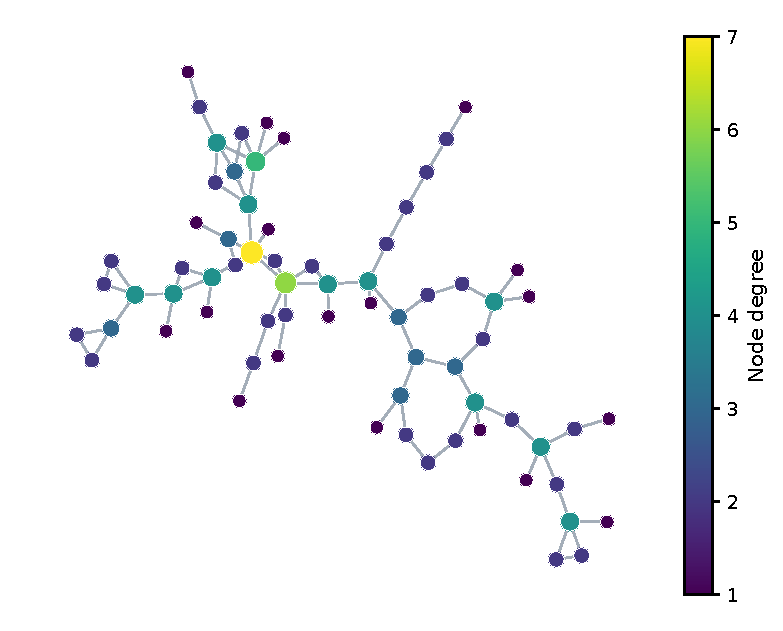
\includegraphics[width=0.72\textwidth]{fig_p2_cc2.pdf}
  \caption{Q4(b): the second largest connected component ($69$ nodes,
  $80$ edges), drawn with a Kamada--Kawai layout. Node size and colour both
  encode degree. Node labels are omitted for legibility.}
  \label{p2:fig:cc2}
\end{figure}

\subsection*{Q4(c): Degree distribution of the whole graph (10 pts)}

Figure~\ref{p2:fig:deg} plots the degree distribution of the \emph{entire}
graph (all $26{,}728$ nodes, not just the giant component). The left panel gives
the raw node count $N(k)$ on linear axes; the right panel gives the fraction of
nodes $P(k)=N(k)/n$ on log--log axes, which is the informative view for a sparse
graph with a heavy tail.

\begin{table}[ht]
  \centering
  \begin{tabular}{lr}
    \toprule
    Degree statistic & Value \\
    \midrule
    Minimum degree & $1$      \\
    Maximum degree & $59$     \\
    Mean degree    & $1.974$  \\
    Median degree  & $1$      \\
    \bottomrule
  \end{tabular}
  \caption{Q4(c): degree statistics over all $26{,}728$ nodes.}
  \label{p2:tab:deg}
\end{table}

\noindent\textbf{Answer.} The degree ranges from a \textbf{minimum of $1$} to a
\textbf{maximum of $59$}, with \textbf{mean degree $1.974$}
($= 2m/n = 2\times 26{,}377/26{,}728$). No node is isolated, since every node
enters the graph through an edge.

The distribution is strongly right-skewed. Degree $1$ alone accounts for
$13{,}942$ nodes ($52.2\%$) and degree $2$ for a further $7{,}423$ ($27.8\%$),
so four fifths of the graph has degree at most $2$; the median degree is $1$.
Only $37$ distinct degree values occur at all, and the tail is thin and ragged
--- the largest degrees ($36$, $38$, $40$, $51$, $57$, $59$) are each realised by
a single node, the maximum being node $22777$ with degree $59$. On log--log axes
the distribution falls off approximately linearly over the bulk of its range
before scattering in the tail, which is the signature of a heavy-tailed,
roughly power-law-like degree distribution rather than a Poisson one. This is
also why the linear panel alone is misleading: on linear axes the whole
distribution collapses into a single spike at $k\le 2$ and the tail out to
$k=59$ is invisible.

\begin{figure}[ht]
  \centering
  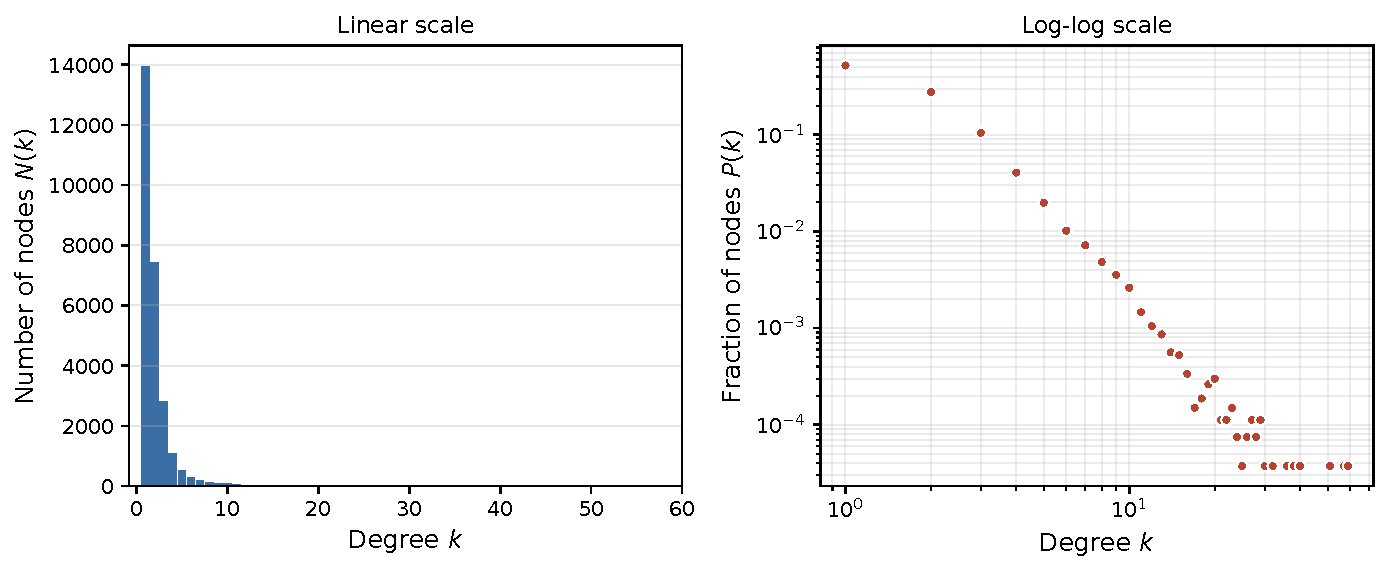
\includegraphics[width=\textwidth]{fig_p2_degree_dist.pdf}
  \caption{Q4(c): degree distribution of the whole graph. Left: node count
  $N(k)$ against degree $k$ on linear axes. Right: the same distribution as a
  fraction of nodes $P(k)$ on log--log axes, which reveals the heavy tail out to
  $k=59$.}
  \label{p2:fig:deg}
\end{figure}
